% ---------------------------------------------------------------------------
% Forward Propagation in a Four-Layer Multilayer Perceptron
% IEEE conference style (two columns, Times, 10 pt) built on the standard
% article class. All numbers come from generated/numbers.tex and all tables
% from generated/*.tex, which are written by make_figures.py.
% ---------------------------------------------------------------------------
\documentclass[10pt,letterpaper,twocolumn]{article}

\usepackage[T1]{fontenc}
\usepackage{mathptmx}
\usepackage[letterpaper,top=0.75in,bottom=1in,left=0.625in,right=0.625in,columnsep=0.25in]{geometry}
\usepackage{amsmath,amssymb}
\usepackage{graphicx}
\usepackage{booktabs,array}
\usepackage{titlesec}
\usepackage[labelsep=period]{caption}
\usepackage{cite}
\usepackage{microtype}
\usepackage{balance}
\usepackage{stfloats}
\usepackage{enumitem}
\usepackage[hidelinks]{hyperref}

\newcommand{\numZManual}{-1.08867}
\newcommand{\numAManual}{0.25187}
\newcommand{\numClassA}{0.25187}
\newcommand{\numOutOne}{0.21184}
\newcommand{\numOutTwo}{0.29902}
\newcommand{\numRandOk}{500}
\newcommand{\numRandN}{500}
\newcommand{\numMaxDiff}{3.3\times 10^{-16}}
\newcommand{\numDefaultMin}{0.203}
\newcommand{\numDefaultMax}{0.312}
\newcommand{\numDemoMin}{0.63}
\newcommand{\numDemoMax}{5.16}
\newcommand{\numHistDefaultMin}{0.203}
\newcommand{\numHistDefaultMax}{0.312}
\newcommand{\numHistDemoMin}{0.48}
\newcommand{\numHistDemoMax}{5.39}
\newcommand{\numExtOne}{0.21094}
\newcommand{\numExtTwo}{0.30027}
\newcommand{\numParams}{68}
\newcommand{\numWOne}{0.47451}
\newcommand{\numWTwo}{0.82380}
\newcommand{\numWThree}{-0.22378}
\newcommand{\numBOne}{-0.05455}
\newcommand{\numBoundDefaultOne}{0.502}
\newcommand{\numBoundDefaultTwo}{0.741}
\newcommand{\numBoundDemoOne}{4.34}
\newcommand{\numBoundDemoTwo}{5.89}
\newcommand{\numZeroOne}{0.0}
\newcommand{\numZeroTwo}{0.11419}


% --- IEEE-like headings ---------------------------------------------------
\renewcommand{\thesection}{\Roman{section}}
\renewcommand{\thesubsection}{\Alph{subsection}}
\titleformat{\section}{\centering\normalfont\small\scshape}{\thesection.}{0.6em}{\MakeUppercase}
\titleformat{\subsection}{\normalfont\small\itshape}{\thesubsection.}{0.6em}{}
\titlespacing*{\section}{0pt}{1.1ex plus 0.3ex minus 0.2ex}{0.8ex}
\titlespacing*{\subsection}{0pt}{0.9ex plus 0.3ex minus 0.2ex}{0.5ex}

% --- IEEE-like captions ----------------------------------------------------
\renewcommand{\thetable}{\Roman{table}}
\captionsetup[figure]{name={Fig.},font=footnotesize,labelsep=period}
\captionsetup[table]{name={TABLE},font=footnotesize,labelsep=newline,textfont=sc,justification=centering}

\setlength{\parskip}{0pt}
\setlist[itemize]{leftmargin=1.2em,itemsep=0pt,topsep=2pt,parsep=0pt}
\setlist[enumerate]{leftmargin=1.5em,itemsep=0pt,topsep=2pt,parsep=0pt}
\pagestyle{plain}

\begin{document}

\twocolumn[{%
\begin{center}
{\fontsize{22}{26}\selectfont Forward Propagation in a Four-Layer Multilayer Perceptron:\\[2pt]
Design, Implementation, and Verification\par}
\vspace{10pt}
{\large Nabonita Das}\\[3pt]
{\small\itshape Course assignment HW\#4 --- Multilayer Perceptron Implementation}\\[1pt]
{\small October 2026}
\vspace{10pt}
\end{center}
}]

\begin{abstract}
\noindent\small\textbf{\textit{Abstract}---}This paper documents the design, implementation and verification of a fully connected multilayer perceptron (MLP) with a 3--5--5--2--2 architecture, in which three sigmoid hidden layers feed a two-neuron ReLU output layer. The network is written from scratch in Python with NumPy and performs forward propagation only; no training is involved. The implementation uses a numerically stable sigmoid, accepts single samples and batches, validates its inputs, and can expose the pre-activation and activation of every layer. Correctness is checked in four independent ways: a hand calculation of one neuron, a second implementation that uses plain loops instead of matrix products, 99 automated tests, and \numRandN{} randomized trials in which both implementations agree to within $\numMaxDiff$. With the default small Xavier-initialised weights, the outputs for 5000 random inputs stay inside a narrow band from \numHistDefaultMin{} to \numHistDefaultMax{}. We show that this band is bounded by the structure of the network, since the last hidden layer lies in the open unit square, and that larger weights widen it to \numHistDemoMin{}--\numHistDemoMax{} without any change to the code.
\end{abstract}

\medskip
\noindent{\small\textbf{\textit{Index Terms}---}multilayer perceptron, feedforward neural network, forward propagation, sigmoid, ReLU, numerical stability, software verification.\par}

\section{Introduction}
Multilayer perceptrons are the simplest neural networks that combine several layers of weighted sums with non-linear activation functions, and they remain the building block inside many larger architectures. Before any learning rule can be applied to such a network, its forward computation must be correct: every prediction, loss value and gradient is derived from the signals that the forward pass produces. This paper therefore concentrates on the forward pass alone and treats it as a piece of software that deserves careful specification and testing.

The network studied here has three input features, three hidden layers of five, five and two neurons with sigmoid activations, and an output layer of two neurons with a rectified linear unit (ReLU). The weights and biases may take any values. We implement the network as a Python class, \texttt{MultilayerPerceptron}, and ask three questions. Is the implementation correct? Is it numerically robust for extreme inputs? And what does the network actually compute when its parameters are small, as they are under a standard initialisation?

The contributions of this paper are as follows.
\begin{itemize}
\item A compact, configurable NumPy implementation of forward propagation with a numerically stable sigmoid, batch support, input validation and a per-layer trace.
\item A layered verification strategy that combines a hand calculation, an independent loop-based implementation, 99 automated tests and 500 randomized trials.
\item An analysis of the output range of the specified network, including a simple provable bound and an experiment that contrasts small and larger weights.
\end{itemize}

Section~\ref{sec:background} reviews the required background. Section~\ref{sec:formulation} states the mathematical model. Section~\ref{sec:impl} describes the implementation, Section~\ref{sec:verification} the verification methods, Section~\ref{sec:results} the results, and Section~\ref{sec:discussion} their interpretation and the limitations of the work.

\section{Background}\label{sec:background}
\subsection{Perceptrons and Multilayer Networks}
The idea of computing with simplified neurons goes back to the threshold units of McCulloch and Pitts~\cite{mcculloch1943}, and Rosenblatt's perceptron~\cite{rosenblatt1958} added a learning procedure for a single layer of such units. Stacking several layers produces a multilayer perceptron, whose weights can be learned by back-propagating error gradients~\cite{rumelhart1986}. A feedforward network with one hidden layer and a suitable non-linear activation can approximate any continuous function on a compact set to arbitrary accuracy when enough hidden units are available~\cite{cybenko1989,hornik1989}. Deeper networks, such as the one in this paper, are used in practice because they often represent useful functions with fewer units~\cite{lecun2015,goodfellow2016}.

\subsection{Activation Functions}
The logistic sigmoid
\begin{equation}
\sigma(z)=\frac{1}{1+e^{-z}}
\end{equation}
maps the real line to the open interval $(0,1)$ and saturates for large $|z|$. The rectified linear unit
\begin{equation}
\mathrm{ReLU}(z)=\max(0,z)
\end{equation}
is zero for negative arguments and the identity otherwise~\cite{nair2010,glorot2011}. Both functions are plotted in Fig.~\ref{fig:act}. Output activations are normally chosen to match the task, for example linear, sigmoid or softmax~\cite{goodfellow2016}. A ReLU at the output, as required here, restricts every prediction to be non-negative and leaves it unbounded above.

\begin{figure}[t]
\centering
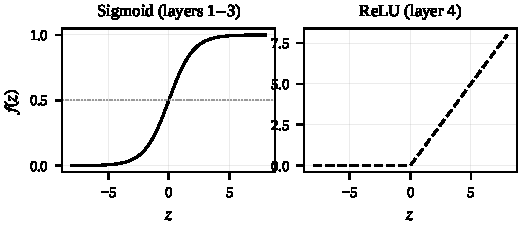
\includegraphics[width=\columnwidth]{figures/fig_activations.pdf}
\caption{The two activation functions used by the network. The sigmoid is applied in layers 1--3 and the ReLU in layer 4.}
\label{fig:act}
\end{figure}

\subsection{Parameter Initialisation}
Without a learning procedure the parameter values are free, but a principled default is still useful. Glorot and Bengio proposed drawing the weights of a layer with $n_\mathrm{in}$ inputs and $n_\mathrm{out}$ outputs uniformly from $[-r,r]$ with $r=\sqrt{6/(n_\mathrm{in}+n_\mathrm{out})}$~\cite{glorot2010}. We use this rule for the weights and a small uniform range for the biases.

\section{Network Architecture and Formulation}\label{sec:formulation}
Let $n_0,\dots,n_4$ be the layer sizes, here $(3,5,5,2,2)$, and let $a^{(0)}\in\mathbb{R}^{1\times 3}$ be the input row vector. Layer $l$ has a weight matrix $W^{(l)}\in\mathbb{R}^{n_{l-1}\times n_l}$, a bias vector $b^{(l)}\in\mathbb{R}^{1\times n_l}$ and an activation function $f_l$. The forward pass computes
\begin{align}
z^{(l)} &= a^{(l-1)}W^{(l)}+b^{(l)},\\
a^{(l)} &= f_l\!\left(z^{(l)}\right),\qquad l=1,\dots,4,
\end{align}
with $f_1=f_2=f_3=\sigma$ and $f_4=\mathrm{ReLU}$, and the network output is $\hat{y}=a^{(4)}\in\mathbb{R}^{1\times 2}$. For a batch of $N$ samples the input becomes a matrix $A^{(0)}\in\mathbb{R}^{N\times 3}$ and the bias is added to every row.

Figure~\ref{fig:arch} shows the connectivity and Fig.~\ref{fig:flow} the resulting data flow. Table~\ref{tab:arch} lists the parameter shapes. The number of trainable parameters is
\begin{equation}
P=\sum_{l=1}^{4}\left(n_{l-1}n_l+n_l\right)=20+30+12+6=\numParams,
\end{equation}
and one forward pass for a single sample needs $15+25+10+4=54$ multiply--accumulate operations and $14$ activation evaluations ($12$ sigmoids and $2$ ReLUs).

\begin{figure*}[t]
\centering
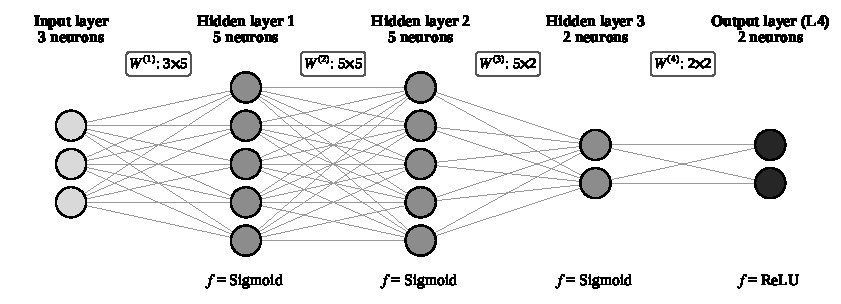
\includegraphics[width=\textwidth]{figures/fig_architecture.pdf}
\caption{Architecture of the 3--5--5--2--2 network. Every neuron is connected to every neuron of the next layer. Boxes give the shape of each weight matrix.}
\label{fig:arch}
\end{figure*}

\begin{figure*}[t]
\centering
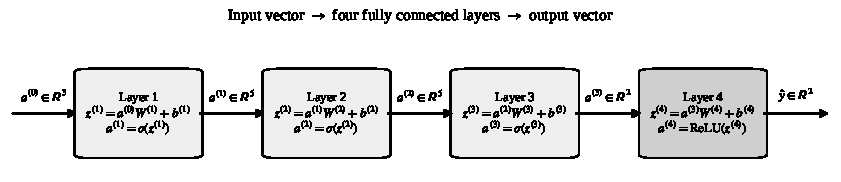
\includegraphics[width=\textwidth]{figures/fig_flow.pdf}
\caption{Data flow of the forward pass. Each block applies an affine map followed by its activation, and the arrows carry the vector dimensions.}
\label{fig:flow}
\end{figure*}

\begin{table}[t]
\caption{Layer Configuration of the Network}
\label{tab:arch}
\centering
\footnotesize
\begin{tabular}{lcccc@{\hspace{6pt}}r}
\toprule
Layer & Neurons & Activation & $W$ & $b$ & Params \\
\midrule
Input & 3 & -- & -- & -- & 0 \\
Hidden 1 (L1) & 5 & Sigmoid & $3\times5$ & 5 & 20 \\
Hidden 2 (L2) & 5 & Sigmoid & $5\times5$ & 5 & 30 \\
Hidden 3 (L3) & 2 & Sigmoid & $5\times2$ & 2 & 12 \\
Output (L4) & 2 & ReLU & $2\times2$ & 2 & 6
\\
\bottomrule
\end{tabular}
\end{table}

\section{Implementation}\label{sec:impl}
\subsection{Software Structure}
The code is organised as shown in Fig.~\ref{fig:soft}. The code is written in Python with NumPy~\cite{harris2020}, and all figures were produced with Matplotlib~\cite{hunter2007}. The module \texttt{multilayer\_perceptron.py} contains the two activation functions and the class. All other files import from it: a demonstration script, a notebook, two test modules and a smoke test. The constructor takes the layer sizes, the activation names, an optional random seed, and optional custom weights and biases. The method \texttt{forward} accepts one sample or a batch and can also return the pre-activation and activation of every layer. A second method, \texttt{forward\_pure\_python}, repeats the computation with plain loops and is used only for verification.

\begin{figure}[t]
\centering
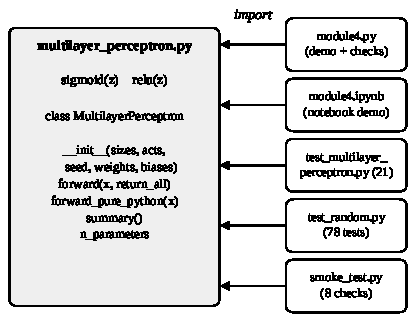
\includegraphics[width=0.80\columnwidth]{figures/fig_software.pdf}
\caption{Software structure. The class lives in one module and is imported by the demonstration script, the notebook and the three test files; numbers give the tests or checks in each.}
\label{fig:soft}
\end{figure}

The core of the forward pass is a loop over the layers:
\begin{verbatim}
for W, b, f in zip(weights, biases, acts):
    z = a @ W + b
    a = f(z)
\end{verbatim}
Because samples are stored as rows, the same code handles a single sample and a batch.

\subsection{Numerically Stable Sigmoid}
Evaluating $1/(1+e^{-z})$ directly overflows the exponential when $z$ is a large negative number. The implementation therefore uses
\begin{equation}
\sigma(z)=\begin{cases}
\dfrac{1}{1+e^{-z}}, & z\ge 0,\\[6pt]
\dfrac{e^{z}}{1+e^{z}}, & z<0,
\end{cases}
\end{equation}
which is algebraically identical but only ever exponentiates a non-positive number.

\subsection{Initialisation and Input Validation}
By default the weights follow the Glorot uniform rule from Section~II-C and the biases are drawn from $[-0.1,0.1]$, using a seeded NumPy random generator so that results are reproducible. Custom weights and biases are accepted if their shapes match the architecture. The class rejects inputs of the wrong rank or feature count and inputs that contain NaN or infinite values, and raises a \texttt{ValueError} with a descriptive message in each case.

\section{Verification Methodology}\label{sec:verification}
\subsection{Hand Calculation}
As a first check, one neuron is computed by hand. For the input $x=(0.5,-1.0,2.0)$ the first neuron of layer 1 has weights $(\numWOne,\ \numWTwo,\ \numWThree)$ and bias $\numBOne$, so
\begin{equation}
\begin{split}
z &= 0.5(\numWOne)-1.0(\numWTwo)\\
  &\quad +2.0(\numWThree)+(\numBOne)=\numZManual,
\end{split}
\end{equation}
and $\sigma(z)=\numAManual$, which equals the value \numClassA{} returned by the class.

\subsection{Independent Implementation}
The method \texttt{forward\_pure\_python} uses only Python lists, loops and the \texttt{math} module. It shares no code with the NumPy path, so agreement between the two is evidence that the vectorised code is correct and not merely self-consistent.

\subsection{Automated Tests}
The test suite has three parts. Twenty-one unit tests cover the architecture, parameter shapes and count, known activation values, stability of the sigmoid for extreme arguments, agreement with a manual calculation, and the error cases. Seventy-eight randomized tests use fixed seeds and draw random inputs of mixed scale, random batches, and random architectures with random weights; they also check that extreme inputs never overflow, that inputs are not modified, and that repeated calls give identical results. A smoke test runs eight quick end-to-end checks. The demonstration script adds seven checks of its own.

\subsection{Randomized Trials}
In addition, \numRandN{} trials were run in which a new network is created from a random seed and evaluated on an input whose scale is $10^{k}$ with $k$ drawn at random from $\{-2,\dots,2\}$. A trial passes if the output is finite, non-negative and equal to the loop-based result within the default tolerance of \texttt{numpy.allclose}.

\begin{table}[t]
\caption{Summary of Verification Evidence}
\label{tab:verify}
\centering
\footnotesize
\begin{tabular}{@{}lcc@{}}
\toprule
Mechanism & Count & Outcome \\
\midrule
Hand calculation (one neuron) & 1 & match, 5 d.p. \\
Unit tests & 21 & all pass \\
Randomized tests (pytest) & 78 & all pass \\
Smoke test & 8 & all pass \\
Script self-checks & 7 & all pass \\
Random trials (NumPy vs.\ loops) & \numRandN{} & \numRandOk{} pass \\
\bottomrule
\end{tabular}
\end{table}

\section{Results}\label{sec:results}
\subsection{A Worked Example}
Table~\ref{tab:trace} shows the full forward pass for the input $(0.5,-1.0,2.0)$ with the default parameters, and Fig.~\ref{fig:layers} plots the activation of each neuron. The final output is $(\numOutOne,\ \numOutTwo)$. In layer 4 the pre-activations are positive, so the ReLU leaves them unchanged and $z^{(4)}=a^{(4)}$.

\begin{table*}[t]
\caption{Layer-by-Layer Trace for the Input $(0.5,-1.0,2.0)$}
\label{tab:trace}
\centering
\footnotesize
\begin{tabular}{@{}clll@{}}
\toprule
Layer & Activation & Pre-activation $z^{(l)}$ & Activation $a^{(l)}$ \\
\midrule
1 & Sigmoid & $-1.089,\ 0.984,\ 0.226,\ 1.999,\ -0.435$ & $0.252,\ 0.728,\ 0.556,\ 0.881,\ 0.393$ \\
2 & Sigmoid & $-0.434,\ -0.016,\ -0.434,\ -0.798,\ 0.651$ & $0.393,\ 0.496,\ 0.393,\ 0.310,\ 0.657$ \\
3 & Sigmoid & $-0.234,\ -0.438$ & $0.442,\ 0.392$ \\
4 & ReLU & $0.212,\ 0.299$ & $0.212,\ 0.299$
\\
\bottomrule
\end{tabular}
\end{table*}

\begin{figure}[t]
\centering
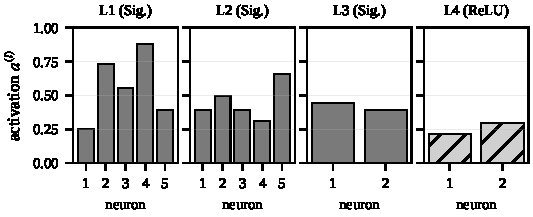
\includegraphics[width=\columnwidth]{figures/fig_layer_activations.pdf}
\caption{Activation of every neuron after each layer for the input $(0.5,-1.0,2.0)$. Sigmoid layers (L1--L3) stay inside $(0,1)$; the ReLU layer (L4, hatched) gives the network output.}
\label{fig:layers}
\end{figure}

\subsection{Further Example Inputs}
Table~\ref{tab:examples} lists the output for five inputs that span zeros, ones, mixed signs, negative values and very large values. The left pair of output columns uses the default parameters and the right pair the larger demonstration weights introduced in Section~VI-\ref{sec:scaled}.

\begin{table*}[t]
\caption{Network Output for Example Inputs}
\label{tab:examples}
\centering
\footnotesize
\begin{tabular}{@{}llcccc@{}}
\toprule
 & & \multicolumn{2}{c}{Default weights} & \multicolumn{2}{c}{Scaled weights} \\
\cmidrule(lr){3-4}\cmidrule(lr){5-6}
Case & Input $(x_1,x_2,x_3)$ & $\hat{y}_1$ & $\hat{y}_2$ & $\hat{y}_1$ & $\hat{y}_2$ \\
\midrule
All zeros & $(0,\ 0,\ 0)$ & 0.21212 & 0.30011 & 3.034 & 4.326 \\
All ones & $(1,\ 1,\ 1)$ & 0.20686 & 0.29293 & 2.463 & 3.627 \\
Mixed & $(0.5,\ -1,\ 2)$ & 0.21184 & 0.29902 & 1.771 & 2.878 \\
Negative & $(-3,\ -2,\ -1)$ & 0.22032 & 0.31186 & 3.436 & 4.782 \\
Large & $(50,\ -50,\ 100)$ & 0.21094 & 0.30027 & 1.221 & 2.241
\\
\bottomrule
\end{tabular}
\end{table*}

\subsection{Behaviour with the Default Weights}
All outputs in Table~\ref{tab:examples} lie between 0.2 and 0.32 for the default network, even though the inputs differ by several orders of magnitude. Figure~\ref{fig:sweep}(a) confirms this: sweeping $x_1$ from $-6$ to $6$ moves each output by less than 0.03. Over 5000 random standard-normal inputs, the outputs stay between \numHistDefaultMin{} and \numHistDefaultMax{} (Fig.~\ref{fig:hist}(a)); the two clusters in that histogram are the two outputs, each concentrated near its own value.

\subsection{Scaled Demonstration Weights}\label{sec:scaled}
To show that this narrow range comes from the parameters and not from the code, a second network is built with the same class. Its weights are drawn from a normal distribution with standard deviation 3.0 (seed 277), and the output-layer weights and biases are made non-negative so that the ReLU neurons stay active. For the same sweep the outputs now range from \numDemoMin{} to \numDemoMax{} (Fig.~\ref{fig:sweep}(b)), and Fig.~\ref{fig:surface} shows a clearly non-linear surface over two inputs, in which a steep transition separates a region of high output from a region of low output. Over 5000 random inputs the outputs span \numHistDemoMin{} to \numHistDemoMax{} (Fig.~\ref{fig:hist}(b)).

\begin{figure}[t]
\centering
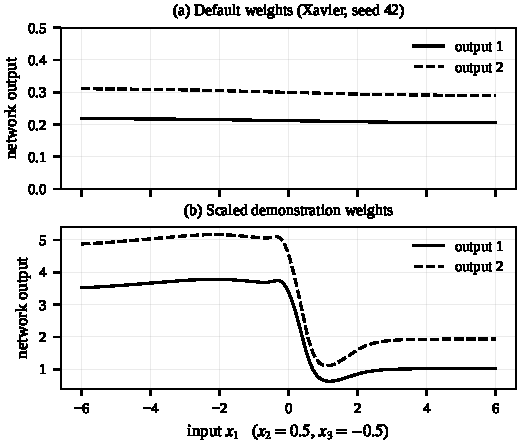
\includegraphics[width=\columnwidth]{figures/fig_sweep.pdf}
\caption{Network output as the first input is swept from $-6$ to $6$ with the other inputs fixed. (a) Default weights: the response is almost flat. (b) Larger demonstration weights: the response is clearly visible.}
\label{fig:sweep}
\end{figure}

\begin{figure}[t]
\centering
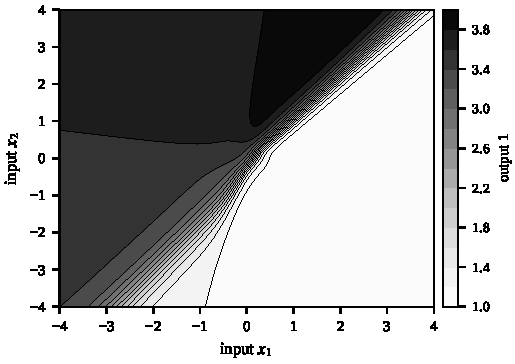
\includegraphics[width=0.78\columnwidth]{figures/fig_surface.pdf}
\caption{Output 1 of the demonstration network over a grid of the first two inputs, with the third input fixed at zero.}
\label{fig:surface}
\end{figure}

\begin{figure}[t]
\centering
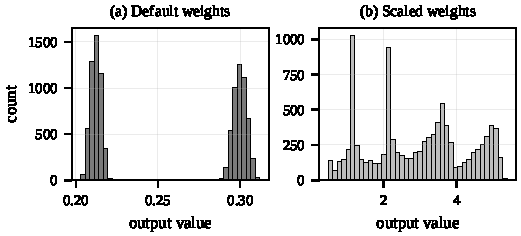
\includegraphics[width=\columnwidth]{figures/fig_hist.pdf}
\caption{Distribution of both outputs over 5000 random standard-normal inputs. (a) Default weights. (b) Scaled weights.}
\label{fig:hist}
\end{figure}

\subsection{Numerical Stability}
With floating-point overflow, invalid-operation and divide-by-zero conditions configured to raise exceptions, the input $(10^{6},-10^{6},10^{6})$ is processed without error and returns $(\numExtOne,\ \numExtTwo)$. These values equal those of the ``large'' input $(50,-50,100)$ in Table~\ref{tab:examples} to five decimal places, which is consistent with saturation of the first-layer sigmoids at 0 or 1.

\section{Discussion}\label{sec:discussion}
\subsection{Why the Default Output Range Is Narrow}
The narrow range is not accidental. The last hidden layer uses a sigmoid, so $a^{(3)}\in(0,1)^2$. Each output is therefore bounded by
\begin{equation}
\hat{y}_j\le\max\!\Big(0,\ \sum_{i}\max\big(W^{(4)}_{ij},0\big)+b^{(4)}_j\Big),
\end{equation}
because every $a^{(3)}_i$ lies between zero and one, so each term $a^{(3)}_iW^{(4)}_{ij}$ is at most $\max(W^{(4)}_{ij},0)$. For the default parameters this gives $\hat{y}_1\le\numBoundDefaultOne$ and $\hat{y}_2\le\numBoundDefaultTwo$, and for the demonstration weights $\hat{y}_1\le\numBoundDemoOne$ and $\hat{y}_2\le\numBoundDemoTwo$. The observed ranges lie inside these bounds. Small weights add a second effect: the pre-activations stay close to the biases, where the sigmoid is nearly linear and varies little. A network of this shape therefore needs larger weights, or an output layer with more freedom, to produce a wide range of outputs.

\subsection{The ReLU Output Layer}
Because the output activation is a ReLU, an output can be exactly zero whenever its pre-activation is not positive, and in that case it carries no information about how negative the pre-activation was. This is illustrated by setting all weights to 0.1, every bias to zero except $b^{(4)}_1=-5$, and using the input $(1,1,1)$; the output is then $(\numZeroOne,\ \numZeroTwo)$. Such behaviour is acceptable for non-negative targets, but it should be kept in mind if the network is later trained, because a neuron that stays at zero receives no gradient.

\subsection{Limitations and Future Work}
The work is limited to the forward pass: the network is not trained, no loss function or back-propagation is implemented, and the demonstration weights were chosen by hand to show a visible response rather than to solve a task. Only dense layers with sigmoid and ReLU activations are supported, and all arithmetic uses 64-bit floating point. Natural extensions are a backward pass verified by numerical gradient checking, further activation functions, and mini-batch training on a small data set.

\section{Conclusion}
A four-layer MLP with a 3--5--5--2--2 architecture, sigmoid hidden layers and a ReLU output layer was implemented from scratch and verified by a hand calculation, an independent loop-based implementation, 99 automated tests and \numRandN{} randomized trials. The implementation is numerically stable for extreme inputs and agrees with the independent version to within $\numMaxDiff$, which is at the level of double-precision rounding. The default small weights produce outputs confined to a narrow band that is bounded by the structure of the network, while larger weights produce a clearly visible response from the same code. These results provide a verified starting point for adding training to the network.

\balance
\begingroup\footnotesize
\begin{thebibliography}{10}
\bibitem{mcculloch1943}
W.~S. McCulloch and W.~Pitts, ``A logical calculus of the ideas immanent in nervous activity,'' \emph{Bull. Math. Biophys.}, vol.~5, no.~4, pp. 115--133, 1943.

\bibitem{rosenblatt1958}
F.~Rosenblatt, ``The perceptron: A probabilistic model for information storage and organization in the brain,'' \emph{Psychol. Rev.}, vol.~65, no.~6, pp. 386--408, 1958.

\bibitem{rumelhart1986}
D.~E. Rumelhart, G.~E. Hinton, and R.~J. Williams, ``Learning representations by back-propagating errors,'' \emph{Nature}, vol.~323, no.~6088, pp. 533--536, 1986.

\bibitem{cybenko1989}
G.~Cybenko, ``Approximation by superpositions of a sigmoidal function,'' \emph{Math. Control Signals Syst.}, vol.~2, no.~4, pp. 303--314, 1989.

\bibitem{hornik1989}
K.~Hornik, M.~Stinchcombe, and H.~White, ``Multilayer feedforward networks are universal approximators,'' \emph{Neural Netw.}, vol.~2, no.~5, pp. 359--366, 1989.

\bibitem{glorot2010}
X.~Glorot and Y.~Bengio, ``Understanding the difficulty of training deep feedforward neural networks,'' in \emph{Proc. 13th Int. Conf. Artif. Intell. Statist. (AISTATS)}, 2010, pp. 249--256.

\bibitem{nair2010}
V.~Nair and G.~E. Hinton, ``Rectified linear units improve restricted Boltzmann machines,'' in \emph{Proc. 27th Int. Conf. Mach. Learn. (ICML)}, 2010, pp. 807--814.

\bibitem{glorot2011}
X.~Glorot, A.~Bordes, and Y.~Bengio, ``Deep sparse rectifier neural networks,'' in \emph{Proc. 14th Int. Conf. Artif. Intell. Statist. (AISTATS)}, 2011, pp. 315--323.

\bibitem{lecun2015}
Y.~LeCun, Y.~Bengio, and G.~Hinton, ``Deep learning,'' \emph{Nature}, vol.~521, no.~7553, pp. 436--444, 2015.

\bibitem{goodfellow2016}
I.~Goodfellow, Y.~Bengio, and A.~Courville, \emph{Deep Learning}. Cambridge, MA, USA: MIT Press, 2016.

\bibitem{harris2020}
C.~R. Harris \emph{et al.}, ``Array programming with NumPy,'' \emph{Nature}, vol.~585, no.~7825, pp. 357--362, 2020.

\bibitem{hunter2007}
J.~D. Hunter, ``Matplotlib: A 2D graphics environment,'' \emph{Comput. Sci. Eng.}, vol.~9, no.~3, pp. 90--95, 2007.
\end{thebibliography}
\endgroup

\end{document}
